\documentclass[tikz,border=12pt]{standalone}
\usepackage[T1]{fontenc}
\usepackage{mathpazo}
\usepackage{amsmath,amssymb}
\usetikzlibrary{arrows.meta, positioning, calc}

\definecolor{stblue}{HTML}{7B97AD}
\definecolor{rwgold}{HTML}{B8995E}
\definecolor{sage}{HTML}{7A9A7E}
\definecolor{dkbrown}{HTML}{3D3530}
\definecolor{wmgray}{HTML}{7B7067}
\definecolor{cream}{HTML}{F9F6F0}
\definecolor{border}{HTML}{D4C9B8}
\definecolor{terracotta}{HTML}{C47A6A}
\definecolor{lavender}{HTML}{907EA0}
\definecolor{rosewood}{HTML}{AD8480}

\begin{document}
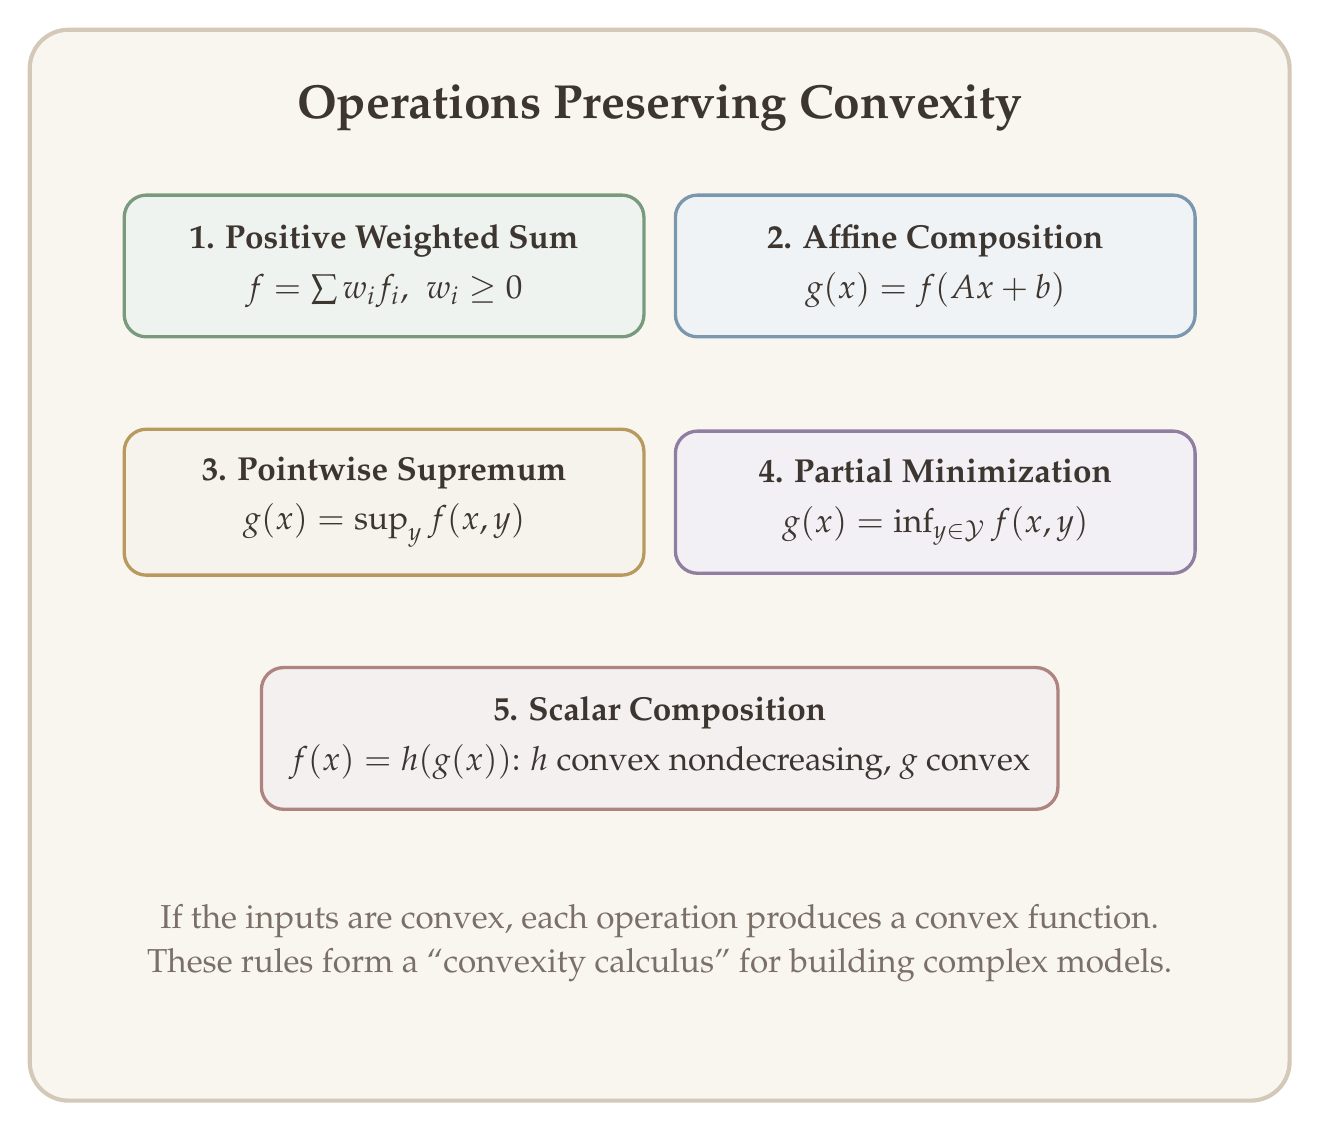
\begin{tikzpicture}[
  every node/.style={text=dkbrown, font=\large},
  opcard/.style={rounded corners=8pt, line width=1.2pt,
    minimum height=1.8cm, minimum width=66mm,
    align=center, text=dkbrown, inner sep=10pt,
    font=\large},
]

% Background
\fill[cream, rounded corners=14pt] (-1.0,-11.8) rectangle (15.0,1.8);
\draw[border, line width=1.5pt, rounded corners=14pt] (-1.0,-11.8) rectangle (15.0,1.8);

% Title
\node[font=\LARGE\bfseries, text=dkbrown] at (7,0.8) {Operations Preserving Convexity};

% 1. Positive Weighted Sum — top left
\node[opcard, fill=sage!12, draw=sage] (op1) at (3.5,-1.2)
  {\textbf{1. Positive Weighted Sum}\\[4pt]
   $f = \sum w_i f_i$,\; $w_i \ge 0$};

% 2. Affine Composition — top right
\node[opcard, fill=stblue!12, draw=stblue] (op2) at (10.5,-1.2)
  {\textbf{2. Affine Composition}\\[4pt]
   $g(x) = f(Ax + b)$};

% 3. Pointwise Supremum — middle left
\node[opcard, fill=rwgold!12, draw=rwgold] (op3) at (3.5,-4.2)
  {\textbf{3. Pointwise Supremum}\\[4pt]
   $g(x) = \sup_{y} f(x,y)$};

% 4. Partial Minimization — middle right
\node[opcard, fill=lavender!12, draw=lavender] (op4) at (10.5,-4.2)
  {\textbf{4. Partial Minimization}\\[4pt]
   $g(x) = \inf_{y \in \mathcal{Y}} f(x,y)$};

% 5. Scalar Composition — bottom center
\node[opcard, fill=rosewood!12, draw=rosewood, minimum width=88mm] (op5) at (7,-7.2)
  {\textbf{5. Scalar Composition}\\[4pt]
   $f(x) = h(g(x))$: $h$ convex nondecreasing, $g$ convex};

% Summary note
\node[font=\large, text=wmgray, align=center] at (7,-9.8)
  {If the inputs are convex, each operation produces a convex function.\\[2pt]
   These rules form a ``convexity calculus'' for building complex models.};

\end{tikzpicture}
\end{document}
